\section{内存页置换机制的执行过程}\label{ux5185ux5b58ux9875ux7f6eux6362ux673aux5236ux7684ux6267ux884cux8fc7ux7a0b}

在lab2/proj8中已经完成了大部分内存页置换所需的功能函数,但还没有有机地整和在ucore中,成为ucore内存管理子系统的组成部分。当有了内核线程机制后,我们就可以把内存页置换的功能整合到一个内核线程中,从而实现一个内存页置换线程kswapd,专门负责完成内存页置换的工作。

\subsection{创建kswapd内核线程}\label{ux521bux5efakswapdux5185ux6838ux7ebfux7a0b}

在第1个内核线程initproc的主体执行函数init\_main中,完成了对kswapd内核线程的创建工作:

\begin{lstlisting}
static intinit_main(void *arg) {    int pid;    if ((pid = kernel_thread(kswapd_main, NULL, 0)) <= 0) {        panic("kswapd init failed.\n");    }    kswapd = find_proc(pid);    set_proc_name(kswapd, "kswapd");
……
\end{lstlisting}

并且保存了创建用户进程前剩余页的情况和已经分配的slab的容量计数,这样在接下来创建完用户进程,并且所有用户进程执行完毕后,再判断所有进程结束后的剩余页的情况和已经分配的slab的容量计数,如果二者相等,这表明内存管理功能基本正确。

\begin{lstlisting}
size_t nr_free_pages_store = nr_free_pages();  size_t slab_allocated_store = slab_allocated();
……
cprintf("all user-mode processes have quit.\n");
……    assert(nr_free_pages_store == nr_free_pages());    assert(slab_allocated_store == slab_allocated());    cprintf("init check memory pass.\n");    return 0;
\end{lstlisting}

\subsection{触发kswapd内核线程}\label{ux89e6ux53d1kswapdux5185ux6838ux7ebfux7a0b}

ucore目前大致有两种触发kswapd内核线程的策略,即积极策略和消极策略。积极策略是指ucore周期性地(或在系统不忙的时候)唤醒kswapd内核线程,让它主动把某些认为``不常用''的页换出到硬盘上,从而确保系统中总有一定数量的空闲页存在,这样当需要空闲页时,基本上能够及时满足需求;消极换出策略是指,ucore试图得到空闲页时,发现当前没有空闲的物理页可供分配,这时才唤醒kswapd内核线程,让kswapd开始查找``不常用''页面,并把一个或多个这样的页换出到硬盘上。

对于积极策略,即每隔1秒唤醒一次内核线程kswapd。在实现上是基于定时器的触发,即在kswapd的主体执行函数kswapd\_main的末尾执行了``do\_sleep(1000);'',这表明了每隔1秒,kswapd就要执行一个回收空闲线程的迭代执行过程。对于消极策略,则是在ucore调用alloc\_pages函数获取空闲页时,此函数如果发现无法从页分配器获得空闲页,就会进一步调用try\_free\_pages来唤醒线程kswapd,让kswapd
换出某些页。在执行try\_free\_pages函数时,由于当前用户进程要求的空闲内存空间无法得到满足,所以首先让当前用户进程睡眠并加入到等待队列中,睡眠原因设置为WT\_KSWAPD,即等待kswapd释放出更多的空闲内存,然后唤醒kswapd:

\begin{lstlisting}
……
        wait_init(wait, current);        current->state = PROC_SLEEPING;        current->wait_state = WT_KSWAPD;        wait_queue_add(&kswapd_done, wait);        if (kswapd->wait_state == WT_TIMER) {            wakeup_proc(kswapd);
……
\end{lstlisting}

\subsection{全局页面置换算法的数据结构设计}\label{ux5168ux5c40ux9875ux9762ux7f6eux6362ux7b97ux6cd5ux7684ux6570ux636eux7ed3ux6784ux8bbeux8ba1}

根据lab2的设计,我们可以知道ucore中表示内存中物理页使用情况的变量是基于数据结构Page的全局变量pages数组,pages的每一项表示了计算机系统中一个物理页的使用情况。如果一个物理页在硬盘上有一个页备份,则ucore需要记录在硬盘中页备份的位置,同时还需要记录swap
分区上的页备份的使用计数。

为了表示物理页可被换出或已被换出的情况,ucore对部分内存相关数据和数据结构进行了扩展。如果一个页被换出了,则页的内容保存在硬盘swap分区上有一个连续扇区中(称为一个swap
page),而对应此页的页表项PTE的Present位为0,表示已经没有对应的物理内存页映射关系了,但如果高24不为0,则表示这个页虽然在物理内存中不存在了,但保存在swap分区中以PTE高24位为偏移位置的swap
page中。这里我们把Present位为0且高24位不为0的PTE称为一个 swap
entry。一个有效的swap entry对应着一个swap page。而且不同页表中的swap
entry可对已一个swap page。

为了表示存储 swap 分区上的页的使用计数,在swap.c 里面声明了全局的
mem\_map 数据结构。如果一个ucore在swap分区上分配了一个

swap.c 里还声明了两个链表,分别是 active\_list 和
inactive\_list,分别表示已经有对应swap
page的且处于``活跃''状态/``不活跃''状态的物理页所形成的链表。所有已经有对应swap
page的物理页page 必须处于两个链表中的一个。

为了更好地对应swap page/swap
entry,在描述物理页的Page数据结构专门设立了几个与页面置换相关的成员变量:

\begin{lstlisting}
struct Page {
    uint32_t flags;   // array of flags that describe the status of the page frame
    swap_entry_t index;      // stores a swapped-out page identifier
list_entry_t swap_link; // swap hash link
……
};
\end{lstlisting}

首先flag的含义做了扩展:

\begin{lstlisting}
// the page is in the active or inactive page list (and swap hash table)
#define PG_swap     4 
// the page is in the active page list
#define PG_active   5
\end{lstlisting}

Page结构中的index值表示物理页在硬盘中页备份的位置,它保存了被换出的页的页表项PTE(即swap
entry)高24位的内容,即硬盘中对应页备份的起始扇区位置值(以扇区为单位)。如果
page数据结构的 flags 设置了PG\_swap 为1,则表示该 page 中的 index
是有效的 swap entry的索引值,从而该物理页上的数据可以被写出到 index
所表示的 swap page 上去。

Page结构中的swap\_link保存了以entry为hash索引的链表项,这样根据entry,就可以快速的对
page
数据结构进行查找。但hash数组在哪里呢?对于在硬盘上有页备份的物理页(简称swap\_page),需要统一管理起来,为此在proj8中就增加了全局变量:

\begin{lstlisting}
static list_entry_t hash_list[HASH_LIST_SIZE];
\end{lstlisting}

hash\_list数组就是我们需要的hash数组,根据 index(swap entry) 索引全部的
swap\_ page 的指针,这样通过hash函数

\begin{lstlisting}
#define entry_hashfn(x)                 (hash32(x, HASH_SHIFT))
\end{lstlisting}

可以快速地根据entry找到对应的page 数据结构。

正如页替换算法描述的那样,把``常用''的可被换出页和``不常用''的可被换出页分别集中管理起来,形成
active\_list 和 inactive\_list 两个链表。
ucore的页面置换算法会根据相应的准则把它认为``常用''的物理页放到active\_list链表中,而把它认为``不常用''的物理页放到inactive\_list链表中。一个标记了
PG\_swap 的页总是需要在这两个链表之间移动。

前面介绍过 mem\_map 数组,他是用来记录 swap\_page 的引用次数的。因为
swap 分区上的 swap page
实际上是某个物理页的数据备份。所以,一个物理页page的 page\_ref 与
对应swap page 的 mem\_map{[}offset{]} (offset = swap\_offset(entry))
值的和是这个页的真实引用计数。page\_ref
表示PTE对该物理页的映射的个数;mem\_map 表示 PTE对该 swap 备份页的
映射个数。当 page\_ref 为0 的时候,表示物理页可以被回收;当
mem\_map{[}offset{]} 为0的时候,表示 swap page
可以被重新存储其他的物理页内容(前面介绍过,可以回收,但是在万不得已的情况下才真的回收)。

\textbf{【注意】}

ucore 目前使用的 PIO 的方式读写 IDE
磁盘,这样的好处是,磁盘读入、写出操作可以认为是同步的,即当前CPU需要等待磁盘读写完毕后再进行进一步的工作。由于磁盘操作相对CPU的速度而言是很慢的,这使得会浪费大量的
CPU 时间在等IO操作上。于是我们总是希望能够在 IO
性能上有更大的提升,比如引入 DMA 这种异步的 IO
机制,为了避免后续开发上的各种不便和冲突,我们假设所有的磁盘操作都是异步的(也包括后面的实验),即使目前是通过
PIO 完成的。

假定某page的 flags中的PG\_swap 标志位为 1,并且PG\_active标志位也为
1,则表示该 page 在 swap 的 active\_list 中,否则在 inactive\_list 中。
active\_list 中的页表示活跃的物理页,即页表中可能存在多个 PTE
指向该物理页(这里可以是同一个页表中的多个
entry,在后面lab3的实验里面有了进程以后,也可以是多个进程的页表的多个
entry);反过来,inactive\_list 链表所链接的 page 通常是指没有 PTE
再指向的页。

\textbf{【注意】}

需要强调两点设计因素:

\begin{enumerate}
\def\labelenumi{\arabic{enumi}.}
\tightlist
\item
  一个 page 是在 active\_list 还是在 inactive\_list 的条件不是绝对的;
\item
  只有 inactive\_list 上的页才会被尝试换出。
\end{enumerate}

这两个设计因素的设计起因如下:

\begin{enumerate}
\def\labelenumi{\arabic{enumi}.}
\tightlist
\item
  我们知道一个 page
  换出的代价是很大的(磁盘操作),并且我们假设所有的磁盘操作都是异步的,那么换出一个
  active 的页就变得非常不值得。因为在还有多个 PTE
  指向他情况下进行换出操作(异步 IO
  可能导致进程切换)的较长过程中,这个页可以随时被其它进程写脏。而硬件提供给内核的接口(即页表项PTE的dirty位)使得内核只能知道一个页是否是脏的(不能明确知道一个页的哪个部分是脏的),当这种情况发生时,就导致了一次无效的写出。
\item
  active\_list 和 inactive\_list 的维护只能由
  与swap有关的集中操作来完成。特别是在lab3/proj11引入
  kswapd内核线程之后,所有的内存页换出任务都交给kswapd,这样减少了复杂的同步互斥实现(在lab5中会重点涉及)。
\item
  页面换入换出有关的操作需要做的就是尽可能的完成如下三件事情:
\end{enumerate}

\begin{itemize}
\tightlist
\item
  将 PG\_swap 为 0 的页转变成 PG\_swap 为1
  的页。即尽可能的给每个物理页分配一个 swap entry(当然前提是有足够大的
  swap 分区)。
\item
  将页从 active\_list 上移动到 inactive\_list 上。如果一个页还在
  active\_list 上,说明还有 PTE
  指向此``活跃''的物理页。所以需要在完成内存页换出时断开对这些物理页的引用,把它变成不活跃的(inactive)。只有把所有的PTE对某page的引用都断开(即
  page的page\_ref 为0)后,就可以将此page从 active\_list 移动到
  inactive\_list 上。
\item
  将 inactive\_list 上的页写出并释放掉。inactive\_list
  上的page表示已没有 PTE
  指向此page了,那么该page可以被释放,如果该page被写过,那还需把此page换出到swap分区上。如果在整个换出过程(异步
  IO)中没有其他进程再写这个物理页(即没有 PTE
  在引用它或有PTE引用但页没有写脏),就认为这个物理页是可以安全释放的了。那么将它从
  inactive\_list 上取下,并调用 page\_free函数 实现 page 的回收。
\end{itemize}

\begin{enumerate}
\def\labelenumi{\arabic{enumi}.}
\setcounter{enumi}{3}
\tightlist
\item
  值得注意的是,内存页换出操作只有特定时候才被调用,即通过
  执行try\_free\_pages函数或者定时器机制(在lab3/proj10.4才引入)定期唤醒kswapd内核线程。这样会导致内存页换出操作对两个链表上的数据都不够敏感。比如处于
  active\_list 上的 page,可能在 kswapd 工作的时候,已经没有 PTE
  再引用它了;再如相应的进程退出了,并且相应的地址空间已经被内核回收,从而变成了一个
  inactive 的 page;还存在inactive\_list 上的 page
  也可能在换出的时候,其它进程通过 page fault,又将 PTE
  指向他,进而变成一个实际上 active 的页。所以说,active 和 inactive
  条件并不绝对。
\end{enumerate}

\subsection{全局页面置换算法的执行逻辑}\label{ux5168ux5c40ux9875ux9762ux7f6eux6362ux7b97ux6cd5ux7684ux6267ux884cux903bux8f91}

其实在lab2/proj8中并没有完全实现页面置换算法,只是实现了其中的部分关键函数,并通过check\_swap来验证了这些函数的正确性。直到lab3的proj11才形成了完整的页面置换逻辑,而这个页面置换逻辑基本上是改进的时钟算法的一个实际扩展版本。

\subsubsection{页状态变化关系}\label{ux9875ux72b6ux6001ux53d8ux5316ux5173ux7cfb}

ucore
采用的页面置换算法是一个全局的页面置换算法,因为它收集了ucore中所有用户态进程(这里可理解为ucore中运行的每个用户态程序)的可换出页,并把这些可换出页中的一部分转换为空闲页。其次它考虑了页的访问情况(根据PTE中PTE\_A位的值)和读写情况(根据PTE中PTE\_D位的值)。如果页被访问过,则把PTE\_A位清零继续找下一页;如果页没有被访问过,这此页就成为了active状态的可换出页,并放入active\_list链表中,这时需要把对应的PTE转换成为一个swap
entry(高24位保存为硬盘缓存页的起始扇区号,PTE\_P位清零);接着refill\_inactive\_scan函数会把处于active状态的部分可换出页转换成inactive状态,并放入inactive\_list链表中;然后page\_launder函数扫描inactive\_list中的处于inactive状态的可换出页,如果此页不是dirty的,则把它直接转换成空闲页,如果此页是dirty的,则执行换出操作,把该页换出到硬盘上保存。这个页的状态变化图如下图所示。

\begin{figure}[htbp]
\centering
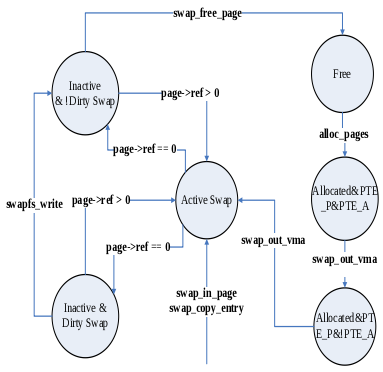
\includegraphics{figures/3.png}
\caption{3}
\end{figure}

ucore的物理页状态变化图

确定腾出的空闲页数和断开的PTE映射数

在proj11中同时实现了积极换出策略和消极换出策略,这都是通过在不同的时机执行kwapd\_main函数来完成的。当ucore调用alloc\_pages函数以获取空闲页,但物理页内存分配器无法满足请求时,alloc\_pages函数将调用try\_free\_pages来通过直接唤醒内核线程kswapd的方式执行kwapd\_main函数,完成对页的换出操作和生成空闲页的操作。这是一种消极换出的策略。另外,ucore也设立了通过设置timer来唤醒线程的方式每秒执行一次kwapd\_main函数,完成对页的换出操作和生成空闲页的操作。这是一种积极换出的策略。

如果alloc\_pages 执行分配 n
连续物理页失败,则会通过调用tree\_free\_page来唤醒kswapd线程。kswapd需要尽可能的满足分配
n 个连续物理页的需求。既然需求是 n 个连续物理页,那么 kswapd
所需要释放的物理页就应该大于 n
个;每个页可能在某个或者许多个页表的不同的地方有 PTE 映射(特别是 copy
on write 之后,这种情况更为普遍),那么 kswapd 所需要断开的 PTE
映射就远远不止 n 个。

Linux 实现了能够根据 physical address
在页表中快速定位的数据结构,但是实现起来过于复杂,这里 ucore
采用了一个比较笨的方法,即遍历所有存在的页表结构,断开足够多的 PTE
映射。这里足够多是个经验公式,采用 n\textless{}\textless{}5
。当然这也可能失败,那么 kswapd
就会尝试一定次数。当他实在无能为力的时候,也就放弃了。而 alloc\_pages
也会不停的调用 try\_free\_pages
进行尝试,当尝试不停的遭遇失败的时候,程序中会有许多句 warn
来输出这些调试信息。而 Linux
的方案是选择一个占用内存最多的进程杀掉并释放出资源,来尽可能的满足当前程序的需求(注意,这里当前程序是指内核服务或者调用),直到程序从内核态正常退出;ucore
的这种设计显然是相对简单了

\subsubsection{页面置换大致流程}\label{ux9875ux9762ux7f6eux6362ux5927ux81f4ux6d41ux7a0b}

kswapd\_main是ucore整个页面置换算法的总控部分,其大致思路是根据当前的空闲页情况查找出足够多的可换出页(swap
page,即page的PG\_swap标志位为1),然后根据这些可换出页的访问情况确定哪些是``常用''页(即page的PG\_swap标志位和PG\_active标志位为1),哪些是``不常用''页,最后把``不常用''的页转换成空闲页。思路简单,但具体实现相对复杂。kswapd腾出更多空闲页的核心是尽可能的断开页表中的
PTE 映射,其整个处理流程分为三步: * 就是把尽可能多的
page(有对应合法PTE项,即对应PTE项的PTE\_P标志位为1) 转变成
具有PG\_active的page(此时的page
PG\_swap标志位和PG\_active标志位都为1,但对应的PTE项的PTE\_P标志位为0),并移动到
active list中; * 接着把 active list
中的页(这些page的PG\_swap标志位和PG\_active标志位为1)尽可能多的变成
inactive list 中页(这些page的PG\_swap标志位为1且PG\_active标志位为0);
* 最后把 inactive list
的页(这些page的PG\_swap标志位为1且PG\_active标志位为0)转换成空闲页,如果这些页是dirty的,则在转换为空闲页之前,先要把页的内容换出(也称为launder,
洗净)到swap分区对应的swap page中。

扫描页表是一项艰巨的任务,因为除了内核空间,用户地址空间有将近 3G
的空间,真正的程序很少能够用这么多。因此,充分利用虚存管理能够提升扫描页表的速度。

\subsubsection{页面置换具体流程}\label{ux9875ux9762ux7f6eux6362ux5177ux4f53ux6d41ux7a0b}

现在我们来介绍以下 kswap\_main 是如何一步一步完成 swap
的操作的。正如前面介绍过的,swap
需要完成3件事情,下面对应的是这三个操作的具体细节:

\paragraph{断开足够多的页表项PTE}\label{ux65adux5f00ux8db3ux591fux591aux7684ux9875ux8868ux9879pte}

kswapd\_main函数通过循环调用函数swap\_out\_mm并进一步调用swap\_out\_vma,来查找ucore中所有存在的虚存空间,并总共断开
m 个 PTE
到物理页的映射。为何是查找ucore中所有存在的虚存空间,而不是直接扫描每个进程的虚存空间呢?这是因为虽然每个用户进程都拥有一个自己的虚存空间,但还存在虚存空间在多个进程之间的共享的情况。所以遍历虚存空间而不是遍历每个进程可避免某个虚存空间被很多进程共享进而被
kswapd
过度压榨所带来的不公平情况。可以想象,被过度压榨的虚存空间,同时又由于被很多进程共享从而有很高的概率被使用到,最终必然会导致频繁的内存访问错误异常\#PF,给系统不必要的负担。

另外虽然 kswapd\_main的第一个任务是断开 m 个 PTE
映射,但是实际上它对每个虚存空间都一次至多提出断开 32
个映射的需求,并循环遍历所有的虚存空间直到 m
得到满足。这样做的目的也是为了保证公平,使得每个虚存空间被交换出去的页的几率是近似相等的。Linux
实际上应该有更好的实现,它根据虚存空间所实际使用的物理页的个数来决定断开的映射的个数。)。这些断开的
PTE 映射所指向的物理页如果没有 PG\_active 标记,则需要给它分配一个新的
swap entry,并做好标记,将 page 插入到 active\_list 中去(同时也插入到
swap 的哈希表中),然后设置好相应的 page\_ref 和 mem\_map{[}offset{]}
的值。

当然,如果找不到空闲的 swap entry 可以分配(比如 swap
分区已经用光了),我们只能跳过这样的 PTE
映射,从下一个地址继续寻找出路;对于原来就已经标记了 PG\_swap
的物理页,则只需要完成后面的工作,即调整引用计数就足够了。

断开的 PTE 被 swap\_entry 取代,并取消 PTE\_P
标记,,这样当出现\#PF的时候,我们能够直接根据 PTE
上的值得到该页的数据实际是在swap 分区上的哪个位置上。

现在这一阶段的工作只是断开 PTE
映射,余下的工作后面会一步步完成。需要注意现在还不必要考虑一个 page
究竟是放在 active\_list 还是放在 inactive\_list
中,也还没涉及页换出操作。当 kswapd 断开足够数量的 PTE
映射以后,第一阶段的工作也就完成了。

当 kswapd 发现自己竭尽所能的遍历都无法满足断开 m
个链接的需求时,该怎么办?我们需要明确的是swap
操作的主要目的是释放物理页,而断开 PTE
映射是一个必要的步骤,作用是尽可能的扩大 inactive\_list 中 page
的个数,为物理页的换出提供更大的基数(操作空间),但这并不是换页主要过程。所以为了防止在这一步陷入死循环,kswapd\_main
最多会对全部虚存空间的链表尝试 rounds=16 次遍。

【注意】虚存管理数据结构mm\_struct新增加了一个 swap\_address
,表示上一次页换出操作结束时的地址。维护这个数据是避免每次 swap
操作都从虚存空间的起始地址开始,从而导致过多数量的重复且无效的遍历。

\paragraph{转换inactive page}\label{ux8f6cux6362inactive-page}

refill\_inactive\_list 从函数名上可以看出,实际上就是遍历
active\_list,把实际上不活跃的(inactive) page 从 active\_list
上取下,放到 inactive\_list 上,方便下一轮 page\_launder 的操作。

\paragraph{页换出和释放页}\label{ux9875ux6362ux51faux548cux91caux653eux9875}

通过 page\_launder 函数,完成遍历
inactive\_list并实现页的释放与换出。page\_launder 的实现,涉及 ucore
内核代码设计的一个重要假设前提,ucore
的内核代码是不可抢占的(具体细节请参考4.5.4小节)。这部分和上述的refill\_inactive\_list
函数操作的先后顺序并不那么严格。通俗的解释就是 page\_launder 实现的是把
inactive\_list 中的 page 洗净(即完成 page
的释放和换出),当然也顺便实现了把实际上活跃的(active) 的 page 从
inactive\_list 上取下,放回 active\_list 的过程。

page\_launder其实是比较复杂的过程,需要仔细的分析一下。page\_launder
先检查一个 page 的 page\_ref 是否 != 0。如果是,则表示该 page 实际上是
active 的,则把它移动到 active\_list
上去;如果不是,则需要对该页进行释放和换出操作。具体过程如下(【注意】下面讨论的是以
page\_ref == 0 作为前提)

\begin{itemize}
\tightlist
\item
  如果一个页的 mem\_map 项为0,说明这个时候已经没有 PTE
  映射指向它了,无论是物理页还是 swap
  备份页。那么这个页也就没有必要洗净了。可以直接释放物理页以及相应的表示为swap
  entry的PTE 了。(同时还需处理 swap page 有关的链表,以下不再赘述)
\item
  如果一个页的 mem\_map 项不为0,但是没有 PG\_dirty 标记:page
  数据结构里面有 PG\_dirty 标记,swap
  部分的代码根据这个标记来判断一个页是否需要被洗净(写到 swap
  分区上)。这个 PG\_dirty
  标记在什么情况下设置,我们稍后会讨论。这种情况可以等价为物理页上的数据和
  swap
  分区上的数据是一致的,所以不需要洗净该页,因为该物理页本身就已经足够干净了。所以可以安全的和(1)
  中的操作一样对该物理页进行释放。
\item
  如果一个页的确有 PG\_dirty 标记:表示该页需要被洗净,这需要调用
  swapfs\_write
  函数,完成将物理页写到磁盘上的操作。前面已经强调过,我们假设所有磁盘操作是异步IO。
  先明确一下,当前的状态,page\_ref=0 \&\&mem\_map!=0 \&\&
  PG\_dirty,那么在执行写到磁盘的过程中就可能发生下面许多种可能的场景:
\end{itemize}

\begin{enumerate}
\def\labelenumi{\alph{enumi}.}
\item
  swapfs\_write
  操作失败了。磁盘操作不像内存操作,它应该允许发生更多的错误。
\item
  其它进程又访问到相应的数据页,前面提到过,因为 PTE
  的PTE\_P标志位为0了,所以会产生\#PF,内核会根据 PTE 的内容在 swap hash
  里面查找到相应的物理页,并将它重新插入到相应的页表中,并更新该 page 的
  page\_ref 和 mem\_map 的值。整个过程发生时,swapfs\_write
  还没有结束。那么当完成洗净一个页的操作时(写到swap 分区),swap
  部分的代码应该有能力检测出这种变化。也就是在 swapfs\_write
  之后,需要再判断 page\_ref 是否依然满足 inactive 的。
\item
  和b类似,不过不同的是,这次对物理页进行的是一个写操作。操作完成之后,进程又将该
  PTE 指向的页释放掉了。那么当 swapfs\_write
  返回的时候,它面对的条件,可能就变成了 page\_ref=0 \&\&mem\_map=0
  \&\&PG\_dirty。它应该能够处理这个变化。
\item
  和c类似,不同的是,该page有两个不同的 PTE 映射。那么在swapfs\_write
  操作之前,状态可能是 page\_ref
  =0\&\&mem\_map=2\&!PG\_dirty,那么当c中的情况发生以后,该物理页的状态就可能变成了
  page\_ref=0\&mem\_map=1\&PG\_dirty了。swap 应该能够处理这种变化。
  综上所述,page\_launder
  部分的代码变得相对复杂很多。大家可以参照程序了解ucore
  是怎么解决这种冲突的。
\end{enumerate}

\subsubsection{其他注意事项}\label{ux5176ux4ed6ux6ce8ux610fux4e8bux9879}

因为 swapfs\_write 是异步操作,并且是对该 page 的操作,ucore
为了保证在操作的过程中,该页不被释放(比如一个进程通过\#PF,增加
page\_ref到1,然后又通过释放该page减少page\_ref到0,进而触发内核执行
page\_free 的操作),分别在 swapfs\_write 前后获得和释放该 page
的引用(page\_ref\_inc/page\_ref\_dec)。但事实证明,这种担心是多余的。理由很简单,当page\_launder
操作一个页的时候,该页是被标记 PG\_swap 的,这个标记一方面表示 page
结构中的 index有意义,另一方面也说明这样的 page 的释放,只能够由 swap
部分的代码来完成(参见 pmm.c 以及后面 shmem.c 的处理)。所以,swap
在操作该 page 的时候,不可能有程序能够调用free\_page释放该 page。

而相反的,mem\_map 是一个需要保护的数据。此外,可以翻阅一下涉及到
page\_ref 修改的 pmm 部分的代码,不难发现,当一个 page 从 PTE
断开的时候,也就是 page\_ref 下降的时候,ucore会根据 PTE 上的硬件设置的
PTE\_D 来设置 PG\_dirty。其实这就足够了。因为 PG\_dirty
并不需要时时刻刻都十分的准确,只要在 swap 尝试判断该 page
是否需要洗净的时候,PG\_dirty 是正确的,就足够了。所以只需要保证每次
page\_ref 下降的时候,PG\_dirty 是正确的即可。除此之外,在对每个页分配
swap\_entry 的时候,需要保证标记
PG\_dirty,因为毕竟是刚刚分配的,物理页的数据还从来没有写出去过。
总结一下,页换入换出的实现很复杂,但是相对独立。并且正是由于 ucore
的内核代码不可抢占使得实现变得相对容易一些。只要是不涉及 IO
操作,大部分过程都可以认为处于不可抢占的内核执行过程。
